\begin{figure*}
    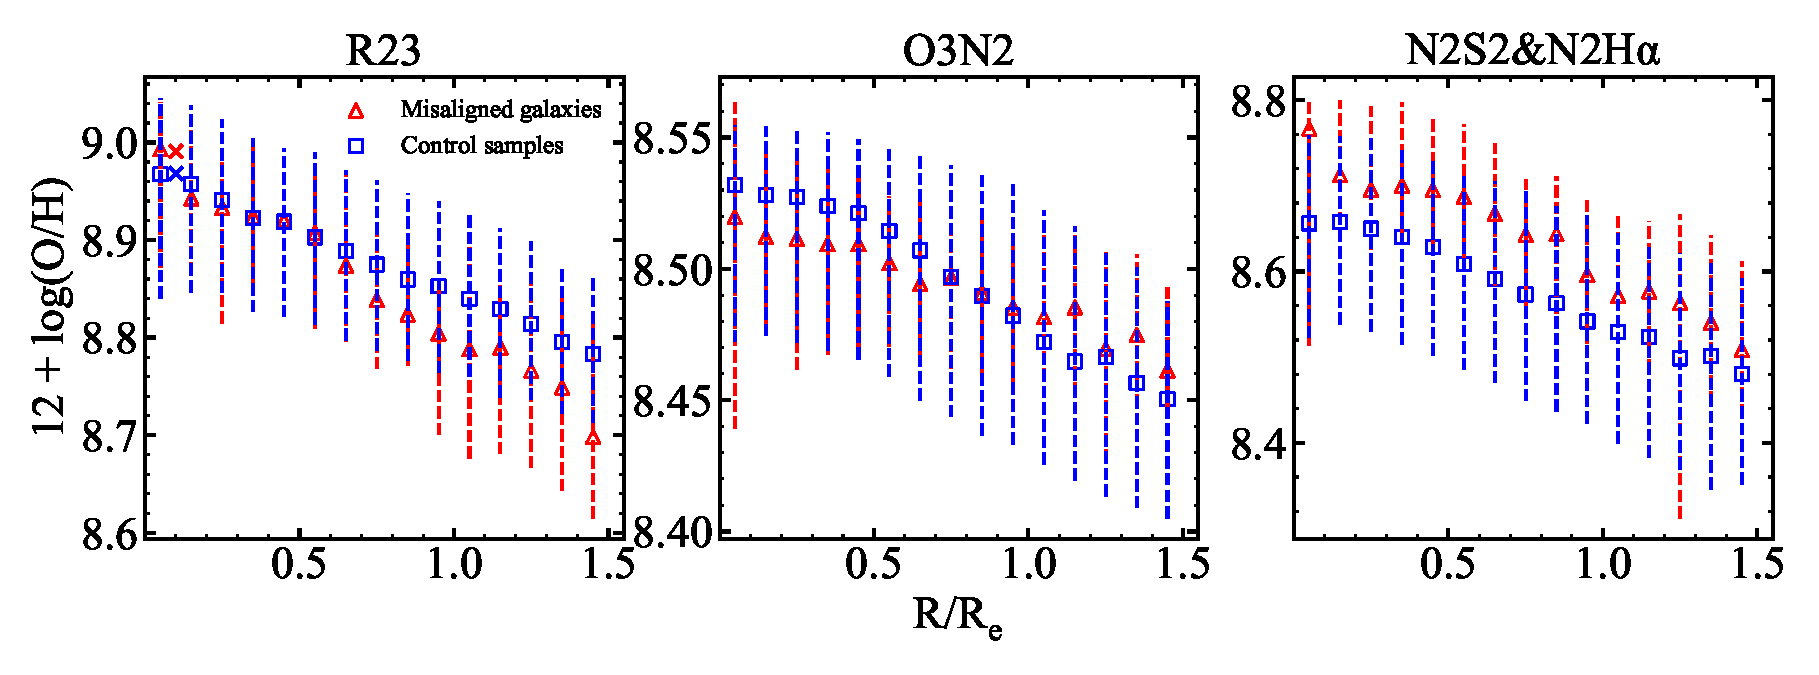
\includegraphics[width=2.0\columnwidth]{pics/SFR_M_control_sample/metallicity.eps}
    \caption{Comparison of gas-phase metallicities estimated from three different strong-line calibrators radial profiles within 1.5 $R_{\rm e}$ between misaligned galaxies and control sample closely matched in SFR and $M_*$. Same as Fig.~\ref{fig:metallicity}, but with the new control sample.}
    \label{fig:metallicity_SFR_M}
\end{figure*}

\begin{figure*}
    
\includegraphics[width=2.0\columnwidth]{pics/SFR_M_control_sample/NII_SII.eps}
    \caption{Comparison of {\nii}$\lambda$6584/{\sii}$\lambda\lambda$6717,6731 radial profiles within 1.5 $R_{\rm e}$ between misaligned galaxies and control sample closely matched in SFR and $M_*$. Same as Fig.~\ref{fig:NII_SII}, but with the new control sample.}
    \label{fig:NII_SII_SFR_M}
\end{figure*}

\begin{figure}
    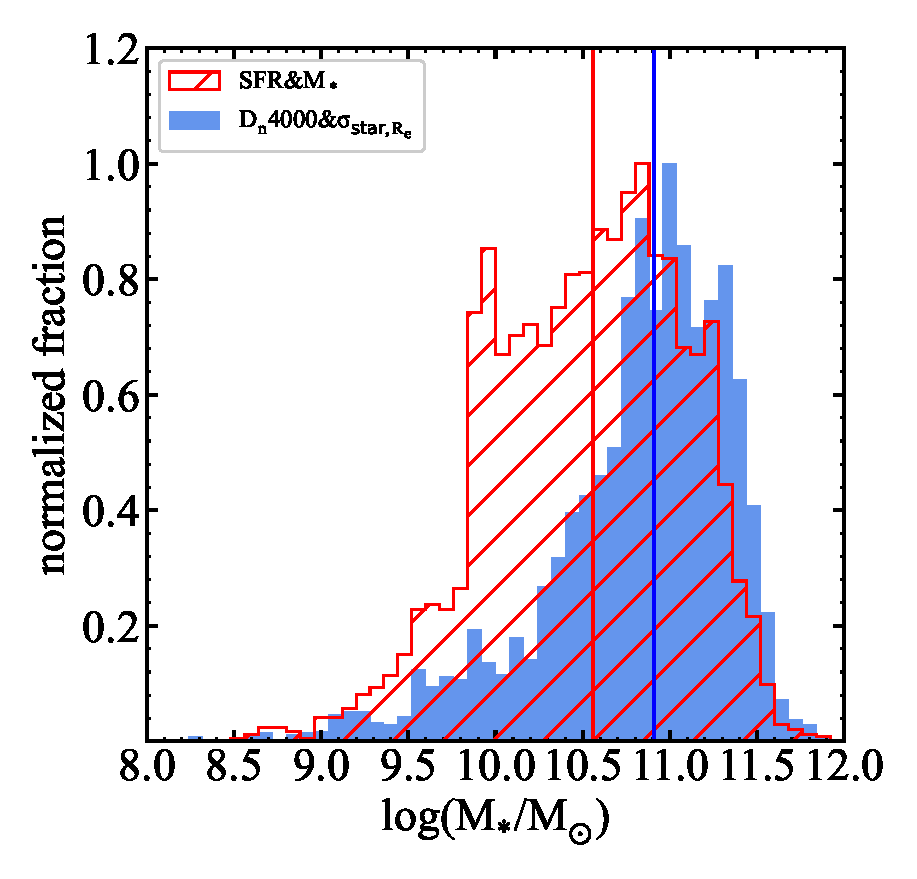
\includegraphics[width=1.0\columnwidth]{pics/SFR_M_control_sample/diff_M.eps}
    \caption{The $M_*$ distribution of control sample closely matched in SFR, $M_*$ (red histograms) as well as control sample closely matched in D$_n$4000, $\sigma_{{\rm star}, R_{\rm e}}$ (blue histograms). The red line is the median $M_*$ of control sample closely matched in SFR, $M_*$ while the blue line is the median $M_*$ of control sample closely matched in D$_n$4000, $\sigma_{{\rm star}, R_{\rm e}}$. The peaks of histogram are set to 1.0.}
    \label{fig:diff_M}
\end{figure}

\section{Discussion}
\label{sec:discussion}

Many previous works have studied the gas-star misalignment phenomena mostly in early type galaxies but rarely in star forming galaxies. Thanks to the large MaNGA sample, \citet{chen_growth_2016} and \citet{jin_sdss-iv_2016} detected gas-star misalignment in star forming galaxies. As a following work of \citet{jin_sdss-iv_2016}, we study the kinematics, stellar populations, star formation activities as well as metallicity of misaligned galaxies, and try to figure out the formation scenarios of misaligned galaxies, as well as how these mechanisms affect the properties of galaxies.

\subsection{Discrepancy in metallicity of SF misaligned galaxies}
\label{sec:discussion-1}
Our results on gas-phase metallicity of GV and QS misaligned galaxies are consistent with previous works \citep{chen_growth_2016, jin_sdss-iv_2016} that GV and QS misaligned galaxies have lower gas-phase metallicity than control samples. At first sight the result on gas-phase metallicity in SF misaligned galaxies seems contrary to previous works. \citet{chen_growth_2016} and \citet{jin_sdss-iv_2016} found SF misaligned galaxies have higher gas-phase metallicity than typical stellar mass-metallicity relation for local star-forming galaxies \citep{tremonti_origin_2004}, but this work finds SF misaligned galaxies have lower gas-phase metallicity than control samples. In this section, we focus on understanding the different results in gas-phase metallicity of SF misaligned galaxies and the dependance of our results on the selection of control samples.

We select another set of ten control samples that are closely match in SFR and $M_*$ with $|\Delta{\rm \log{SFR}}| \leq 0.2$ and $|\Delta{\log{M_*}}| \leq 0.1$, we repeat Fig.~\ref{fig:vel_divide_sigma} to Fig.~\ref{fig:NII_SII} based on the new control samples, finding that all the results are consistent with previous sections except the gas-phase metallicity of SF misaligned galaxies. Fig.~\ref{fig:metallicity_SFR_M} shows gas-phase metallicity estimated from three different strong-line calibrators for misaligned galaxies and the new control samples. The metallicity of the central region traced by $R_{23}$, N2S2\&N2$\ha$ and $\nii\lambda6584/\sii\lambda\lambda6731,6717$ is higher in misaligned galaxies than control samples, which is opposite to Fig.~\ref{fig:metallicity} and \ref{fig:NII_SII}. The central metallicity estimated from O3N2 of misaligned galaxies is still slightly lower than that of control sample. The red and blue crosses in the left panel of Fig.~\ref{fig:metallicity_SFR_M} mark the median value of central $3^{\prime \prime}$ gas-phase metallicity from MPA-JHU catalogue for misaligned galaxies and control samples. Our gas-phase metallicity in the central region is totally consistent with that from MPA-JHU catalogue. The central metallicity estimated from $R_{23}$ is $\sim$0.03 dex higher in the SF misaligned galaxies than control samples selected by SFR, $M_*$, but $\sim$0.03 dex lower than control samples closely matched in total D$_n$4000, $\sigma_{{\rm star}, R_{\rm e}}$ (left panel of Fig.~\ref{fig:metallicity}).

In order to understand the different results of gas-phase metallicity, we investigate the properties of different control samples. Fig.~\ref{fig:diff_M} shows the $M_*$ distribution of the two sets of control samples, it is clear that the $M_*$ of control samples selected by total D$_n$4000 and $\sigma_{{\rm star}, R_{\rm e}}$ is $\sim$0.35 dex larger than that of control sample selected by SFR, $M_*$. This $\sim$0.35 dex difference in $M_*$ is large enough to explain the $\sim$0.06 dex difference in metallicity between the two sets of control samples. SF misaligned galaxies do not follow the typical $M_*-\sigma_{{\rm star}, R_{\rm e}}$ relation. They have smaller $M_*$ than control sample closely matched in $\sigma_{{\rm star}, R_{\rm e}}$, but have larger $\sigma_{{\rm star}, R_{\rm e}}$ than control sample closely matched in $M_*$. Why the SF misaligned galaxies are the outliers in the $M_*-\sigma_{{\rm star}, R_{\rm e}}$ relation, one possibility is that the newly formed stars inherited the angular momentum of accreted gas that was not consistent with pre-existing stars, the contribution of these two parts of stars could broaden the observed stellar velocity dispersion, similar to 2$\sigma$ galaxies \citep{krajnovic_atlas3d_2011}. Limited by MaNGA spectral resolution, we can not clearly distinguish multiple stellar components with different line of sight velocity, future observations of higher spectral resolution are required to figure out this possibility.

\subsection{Formation scenarios of misaligned galaxies}
\label{sec:discussion-2}

In the last decades, several formation scenarios of gas-star misalignments have been proposed, including external gas accretion from dwarf companions as well as cosmic webs \citep{1998ApJ...506...93T, chen_growth_2016, jin_sdss-iv_2016}, minor/major mergers \citep{naab_atlas3d_2014, li_impact_2020}. Recent simulations \citep{starkenburg_origin_2019, duckworth_decoupling_2020, koudmani_little_2021} find a higher incidence of AGN in misaligned galaxies, suggesting AGN feedback also plays a role in the formation of misalignment.

In this work, we suggest that from SF to QS, these different types of galaxies have survived from different formation scenarios. \citet{chen_growth_2016} and \citet{jin_sdss-iv_2016} proposed that in the SF misaligned galaxies, the interaction between accreted gas and pre-existing gas leads to the consumption of angular momentum, large amount of gas flows to the central regions of galaxies, triggering the central star formation/starburst. Our results for SF galaxies in Fig.~\ref{fig:vel_divide_sigma} to Fig.~\ref{fig:SFR_and_sSFR} totally support this picture. The lower $V_{\rm gas}/{\sigma}_{\rm gas}$ and $V_{\rm star}/{\sigma}_{\rm star}$ of the misaligned galaxies than the control samples are due to angular momentum loss, lower D$_n$4000 and light-weighted ages, as well as higher $\Sigma_{\rm SFR}$ and sSFR at the central regions of SF misaligned galaxies are consistent with central star formation. We suggest that the primary formation mechanisms for SF misaligned galaxies is external gas accretion. The results for GV misaligned galaxies from Fig.~\ref{fig:vel_divide_sigma} to Fig.~\ref{fig:lw_age_and_mw_age} show similar trend as SF misaligned galaxies, suggesting the GV misaligned galaxies have undergone similar formation mechanisms as the star forming misaligned galaxies. On the other hand, most SF and GV misaligned galaxies show spiral or S0-like morphology. Numerical simulations suggest that mergers, especially major mergers can hardly keep the disk structure in spiral or S0 galaxies \citep{1992ApJ...393..484B} except in some extreme conditions, such as a major merger with a spiral-in falling \citep{zeng_formation_2021}.

For the QS misaligned galaxies, they show obvious difference from SF and GV galaxies. Although QS misaligned galaxies also have lower $V_{\rm gas}/{\sigma}_{\rm gas}$ and $V_{\rm star}/{\sigma}_{\rm star}$ than the control galaxies, the difference is much smaller than that in SF, GV. There is evidence that the QS misaligned galaxies have older stellar populations than the control samples as suggested by D$_n$4000, light- and mass-weighted ages. We suggest there are three different formation mechanisms for QS misaligned galaxies: (1) QS misaligned galaxies are the evolutionary results of GV galaxies; (2) merger contribution is larger in QS misaligned galaxies than SF and GV misaligned galaxies. \citet{li_impact_2020} find merger fraction is $\sim$10\% higher in QS misaligned galaxies than the co-rotating counterparts, while the difference in merger fraction between SF, GV misaligned galaxies and their co-rotating counterparts is not obvious; (3) the QS misaligned galaxy is formed through gas accretion by a gas-poor elliptical galaxy and this gas accretion process does not influence the evolution of progenitors. In this case, progenitors with less gas, much older stellar populations are easier to show misaligned phenomena since the interaction between accreted and pre-existing gas can be neglected, it is easier for the accreted gas to keep their original angular momentum. In this scenario, the observed difference between QS misaligned galaxies and their control galaxies is totally due to the difference between the progenitors.

A new class of elliptical galaxy termed as `red geyser' has been identified from MaNGA \citep{2016Natur.533..504C}. These `red geysers' are believed to exhibit high velocity outflow triggered by AGN. And the misaligned phenomenon is prevalence in `red geysers'. Based on cosmological simulations, \citet{starkenburg_origin_2019}, \citet{duckworth_decoupling_2020} and \citet{ koudmani_little_2021} investigated the impact of AGN feedback on the formation of low-mass misaligned galaxies, suggesting that low-mass misaligned galaxies tend to have increased AGN feedback and increased energy injection, which leads to the removal of pre-existing gas and further reduces the interaction between accreted and pre-existing gas, follow up external gas accretion leads to the gas-star misaligned phenomenon. In this work, we also find that the AGN fraction is 2-3 times higher in the SF and GV misaligned galaxies than their control samples, however, we would like to trust this as a nature result of gas inflow. The gas inflow on the one hand triggered the central star formation, on the other hand provided fuels for the central BHs, leading to a higher AGN fraction. The gas removal scenario suggested by the literatures can not explain the enhanced central star formation in SF and GV misaligned galaxies. For the QS misaligned galaxies, we do not find any obvious difference in AGN fraction between the misaligned and control samples.
